\section{Exemple: quelques variations sur le thème des éléments unidimensionnels}

Dans ce paragraphe, nous appliquons ce que nous venons de voir sur quelques cas simples d'éléments unidimensionnels.

\medskipvm
\subsection{Élément de référence unidimensionnels linéaire à deux nœuds}\label{Sec-Elt1D2}

Considérons un segment reliant deux points dans l'espace. Ce segment est défini par un point courant dont les coordonnées sont le vecteur~$\VV{x}$. On peut paramétrer ce segment par le paramètre~$\xi \in [-1,1]$, et le vecteur position s'exprime par~$\LL{x}=\LL{x(\xi), y(\xi), z(\xi)}$.
\begin{figure}[ht]\centering\small
   \subfloat[Élément de référence]{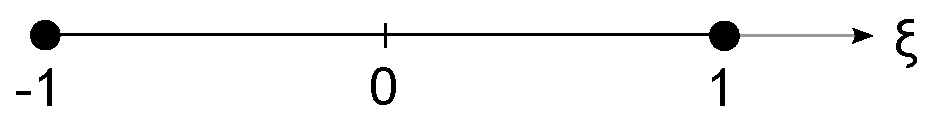
\includegraphics[width=60mm]{Elt1D-ref.eps}} \hspace{5em}
   \subfloat[Segment réel (3D)]{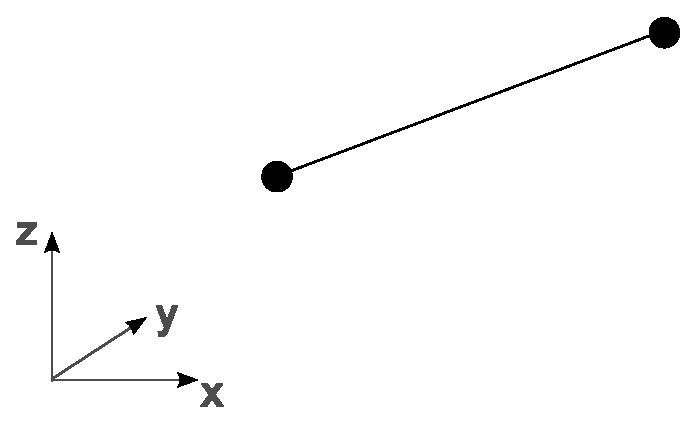
\includegraphics[width=40mm]{Elt1D-espace.eps}}
   \caption{Correspondance entre élément de référence et géométrie réelle}\label{fig-e1rr}
\end{figure}
\medskipvm
Cet élément (segment) est défini par ses seules extrémités. Nous avons donc deux nœuds de coordonnées~$\LLP{x_1, y_1, z_1}$ et~$\LLP{x_2, y_2, z_2}$.
\medskipvm
Un point courant de cet élément sera obtenu par interpolation linéaire entre les deux nœuds, paramétrée par~$\xi$. On Cherche cette interpolation sous la forme~$x(\xi)=\LL{N(\xi)}\VV{x_n}$, $y(\xi)=\LL{N(\xi)}\VV{y_n}$ et~$z(\xi)=\LL{N(\xi)}\VV{z_n}$, avec
$\LL{N(\xi)}=\LLL{N_1(\xi), N_2(\xi)}$ et~$N_1(\xi)=\frac12 (1-\xi)$, $N_2(\xi)=\frac12(1+\xi)$.
De manière plus «compacte», on peut écrire:
\begin{equation} N_i(\xi)=\frac12(1+\xi_i\xi), \qquad i=1,2, \quad \xi_i=\pm1 \quad (\text{et } \xi\in[-1,1]) \end{equation}
\medskipvm
Dans cette interpolation (comme dans toutes interpolation), on a une relation entre~$\dd\VV{x}$ et $\dd\xi$. Notons~$\dd\VV{x} = \VV{a} \dd \xi$. Alors:
\begin{equation} \LL{a} = \LLL{x_{,\xi}, y_{,\xi}, z_{,\xi}} = \frac12 \LLL{x_{21}, y_{21}, z_{21}}\end{equation}
avec ici~$x_{21}=x_2-x_1$, $y_{21}=y_2-y_1$ et~$z_{21}=z_2-z_1$.
On voit ainsi comment passer d'une intégrale sur le segment réel à une intégrale sur l'élément de référence.

\medskipvm
De même, on peut chercher la relation entre~$\dd s=\dd\VV{x}\cdot\dd\VV{x}$. Nous notons $\dd s=m \dd \xi$. On a alors: 
\begin{equation}m=|\VV{a}| = \frac12 \sqrt{x_{21}^2+y_{21}^2+z_{21}^2} = \frac{L_e}2 \end{equation}
On voit alors l'égalité des intégrations:
\begin{equation}\int_{L_e} \ldots \dd s = \int_{-1}^{+1}\ldots m \dd \xi\end{equation}

\medskipvm
Par ailleurs, on a la relation:
\begin{equation} \frac{\dd}{ \dd \xi} = \frac{\dd s}{ \dd \xi}\frac{\dd}{\dd s}=m\frac{\dd}{\dd s}\end{equation}

\medskip
\subsection{Rappels sur la jacobienne et le jacobien d'une transformation}\index{jacobien}\index{jacobienne}

Nous considérons une transformation de~$\RR^n$ dans~$\RR^m$ donnée par la fonction~$f$: 
$\left(x_1, \ldots, x_n \right) \mapsto \left(f_{y_1}, \ldots, f_{y_m} \right)$.
\medskipvm
La \textcolorblue{matrice jacobienne}\index{jacobienne} (d'après Carl Jacobi)\index[aut]{Jacobi (Carl Gustav Jakob), 1804-1851, Allemand} associée à~$f$ est définie par:
\begin{equation}
J_f = \MM*{\LL{\nabla f_{y_1}} \\ \vdots \\ \LL{\nabla f_{y_m}}}
\end{equation}
i.e., sous forme complètement développée la jacobienne de~$f$ s'écrit:
\begin{equation}
J_f = \MM*{\frac{\partial f_{y_1}}{\partial x_1} & \cdots & \frac{\partial f_{y_1}}{\partial x_n} \\ \vdots & \ddots & \vdots \\ \frac{\partial f_{y_m}}{\partial x_1} & \cdots & \frac{\partial f_{y_m}}{\partial x_n}}
\end{equation}
\medskipvm
Au voisinage d'un point~$M$, l'approximation linéaire de la fonction~$f$ est donnée par:
\ifVersionDuDocEstVincent
\begin{equation} f\left(X\right) \approx f\left(M\right) + J_f\left(M\right) \overrightarrow{MX}\end{equation}
\else
\begin{equation} f\left(X\right) \approx f\left(M\right) + J_f\left(M\right) \mathbf{MX}\end{equation}
\fi
\medskipvm
La composée~$f\circ g$ de fonctions différentiables est différentiable, et sa matrice jacobienne s'obtient par la formule:
\begin{equation} J_{f \circ g}= \bigl( J_f \circ g \bigr) \cdot J_g\end{equation}
\medskipvm
Dans le cas où \textcolorred{$m = n$}, on appelle~$j_f$ le \textcolorblue{jacobien}\index{jacobien} de~$f$, 
défini comme le déterminant de sa matrice jacobienne: \index{jacobien}\index{jacobienne}
\begin{equation} j_f = \det\, \left(J_f \right) \end{equation}
Dire que le jacobien est non nul revient donc à dire que la matrice jacobienne est inversible.
\medskipvm
Si le jacobien\index{jacobien} est positif au point~$M$, l'orientation de l'espace est conservée au voisinage de ce point. À l'inverse, l'orientation est inversée si le jacobien est négatif.
\medskipvm
Le jacobien\index{jacobien} d'une composée de fonctions est le produit des jacobiens individuels.
\medskipvm
Le jacobien\index{jacobien} de la réciproque d'une fonction est l'inverse du jacobien de la fonction.
\medskipvm
\colorgris
Cette dernière propriété est liée au théorème d'inversion locale (qui peut être vu entre autre comme une extension du théorème des fonctions implicite en dimension supérieure à 1 dans le cas réel).
\medskipvm
Une fonction~$F$ de classe~$C^1$ est inversible au voisinage de~$M$ avec une réciproque~$F^{-1}$ 
de classe~$C^1$ si et seulement si son jacobien en~$M$ est non nul (théorème d'inversion locale). De plus, la matrice jacobienne de~$F^{-1}$ se déduit de l'inverse de la matrice jacobienne de~$F$ au moyen de la formule:\index{jacobien}\index{jacobienne}
\begin{equation}J_{F^{-1}} = \bigl( J_F \circ F^{-1} \bigr)^{-1}\end{equation}

\begin{theoreme}[Théorème d'inversion locale]\index{théorème!d'inversion locale}
Soit~$f$ une application de~$U$ dans~$F$, où~$U$ est un ouvert d'un espace de Banach réel et $F$ un espace de Banach et soit~$x$ un point de~$U$.
Si~$f$ est de classe~$C^p$, avec~$p$ un entier strictement positif et si la différentielle de~$f$ au point $x$ est un isomorphisme bicontinu, alors il existe un voisinage ouvert~$V$ de~$x$ et un voisinage ouvert $W$ de~$f(x)$ tels que~$f$ se restreigne en une bijection de~$V$ dans~$W$ dont la réciproque est de classe~$C^p$.
\end{theoreme}
\colorblack
\medskipvm
\textcolorgreen{Comme illustré au paragraphe précédent, le jacobien sert surtout pour effectuer des changement de variables dans le calculs des intégrales.}
\medskipvm
\begin{theoreme}[Théorème de changement de variables dans les intégrales multiples]\index{théorème!de changement de variables dans les intégrales multiples}
Soient~$U$ un ouvert de~$\RR^n$, $F$ une injection de classe~$C^1$ de~$U$ dans~$\RR^n$ et~$V=F(U)$.

Si~$g$ est une fonction mesurable de~$V$ dans~$\intfo{0}{+\infty}$, on a égalité des intégrales pour la mesure de Lebesgue sur~$\RR^n$:
\begin{equation}  \int_V g(y_1,\ldots,y_n)~\dd y_1\ldots\dd y_n = \int_U g\left(F\left(x_1,\ldots,x_n\right)\right) 
\left|\det J_F(x_1,\ldots,x_n)\right|~\dd x_1\ldots\dd x_n.
\end{equation}
\end{theoreme}
\medskipvm
\textcolorgreen{Si l'on considère un «petit» domaine, le volume de l'image de ce domaine par la fonction~$f$ sera celui du domaine de départ multiplié par la valeur absolue du jacobien.}\index{jacobien}

\medskip
\subsection{Éléments de référence unidimensionnels linéaires à~$n$ nœuds}

Il est possible de généraliser en considérant un segment ayant plusieurs nœuds intermédiaires comme indiqué sur la figure~\ref{fig:ex2:noeudint}.
\begin{figure}[ht]\centering
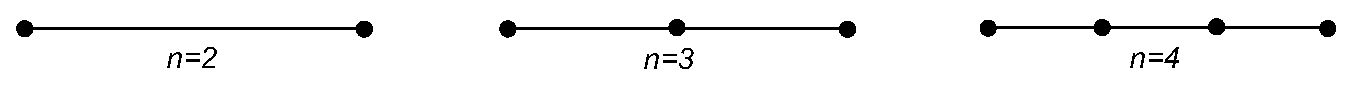
\includegraphics[width=140mm]{Elt1D-ex.eps}
\caption{Nœuds intermédiaires}\label{fig:ex2:noeudint}
\end{figure}
\medskipvm
Si l'on considère le cas général à~$n$ nœuds de la figure~\ref{fig:ex2:casgen}
\begin{figure}[ht]\centering
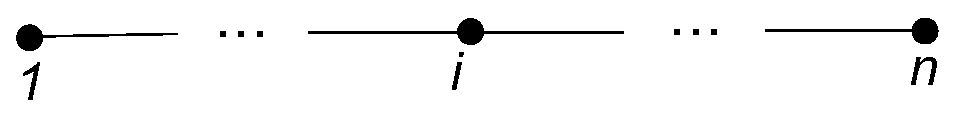
\includegraphics[width=60mm]{Elt1D-n.eps}
\caption{Cas général}\label{fig:ex2:casgen}
\end{figure}
alors il vient:
\begin{equation} N_i(\xi) = \prod_{r=1\atop r\ne i}^n \dfrac{\xi_r-\xi}{\xi_r-\xi_i} \end{equation}
\medskipvm
Si de plus, les~$n$ nœuds sont régulièrement espacés:
\begin{equation}\xi_i = -1+2\frac{i-1}{n-1} \qquad
N_i(\xi) = \prod_{r=1\atop r\ne i}^n \dfrac{(2r-n-1)-\xi(n-1)}{2(r-i)} \end{equation}

\medskip
\subsection{Élément de référence unidimensionnel infini}

Dans certains cas, il peut être nécessaire de prendre en compte des conditions aux limites situées à l'infini: problèmes de fondations, d'acoustique, de couplage fluide-structure.

Il est possible, comme aux paragraphes précédents, de proposer une transformation entre un élément de référence de longeur 2 et un élément réel infini, transformation illustrée sur la figure~\ref{fig:ex2:trans}.
\begin{figure}[ht]\centering
\begin{tabular}{cc}
\subfloat[Élément de référence]{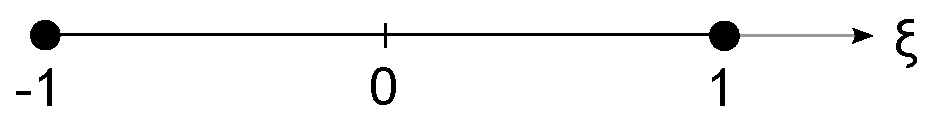
\includegraphics[width=65mm]{Elt1D-ref.eps}} \hspace{5em}
\subfloat[Élément réel (infini)]{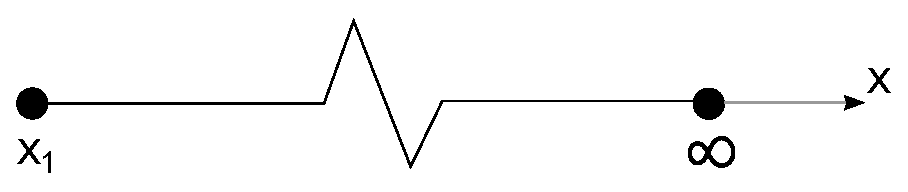
\includegraphics[width=65mm]{Elt1D-infty.eps}}
\end{tabular}\caption{Correspondance entre l'élément de référence et l'élément réel infini}\label{fig:ex2:trans}
\end{figure}
\medskipvm
Nous ne considèrerons que le cas de l'élément unidimensionnel linéaire à 2 nœuds dans ce paragraphe, mais on pourrait étudier le cas de l'élément linéaire unidimensionnel à~$n$ nœuds, ou des éléments bidimensionnels par exemple.
\medskipvm
Nous allons toujours avoir une interpolation de la fonction solution sous la forme:
\begin{equation} u =\frac{1-\xi}2 u_1 + \frac{1+\xi}2 u_2\end{equation}
car concrètement~$u_2$ est connu (et fini): c'est le «lieu» où l'on situe l'infini dans le modèle éléments finis.
\medskipvm
Par contre, l'interpolation du point courant sera donnée par:
\begin{equation}
x=x_1+\frac{1+\xi}{1-\xi}\alpha
\end{equation}
où~$\alpha$ est une constante.
\medskipvm
On aura également:
\begin{equation} u_{,x} = \frac{u_2-u_1}{4\alpha} (1-\xi)^2 \end{equation}

\medskip
\subsection{Élément fini de barre unidimensionnel}\label{Sec-barre1D}

On considère la barre de la figure~\ref{fig-barre}, de section~$A$, de longueur~$L$, et constituée d'un matériau homogène isotrope de module d'Young\index[aut]{Young (Thomas), 1773-1829, Anglais}\index{module d'Young} $E$ et densité~$\rho$ et soumise uniquement à son poids propre.
\begin{figure}[ht]
\centering
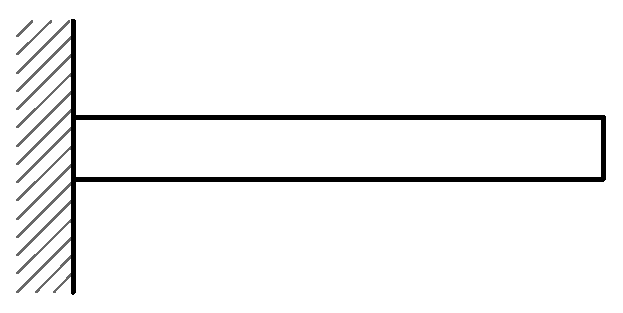
\includegraphics[width=40mm]{Elt1D-barre.eps}
\caption{Barre encastrée-libre}\label{fig-barre}
\end{figure}
On souhaite discrétiser ce problème à l'aide d'un éléments unidimensionnels linéaires
tel que présenté au paragraphe~\ref{Sec-Elt1D2}.
\medskipvm
La forme variationnelle de ce problème d'élasticité linéaire unidimensionnel (théorie des poutres) est:
\begin{equation}
W=\dint_0^L EA v_{,x}u_{,x} \dd x - \dint_0^L \rho g A v = 0, \quad \forall v
\end{equation}
avec les conditions aux limites~$u(0)=0$ et~$v(0)=0$.
Cette forme variationnelle, s'écrit pour l'élément (ou pour chaque élément si on en avait plusieurs):
\begin{equation}
W = \LL{v} \left( \MM{K}\VV{u} - \VV{f} \right)
\end{equation}
\medskipvm
Nous avons vu que la géométrie, représentée par un élément, est approximée par:
\begin{equation} x=\frac{1-\xi}2 x_1 + \frac{1+\xi}2 x_2, \quad \xi\in[-1;1] \end{equation}
La représentation de la fonction solution, est:
\begin{equation} u = \frac{1-\xi}2 u_1 + \frac{1+\xi}2 u_2, \quad \xi\in[-1;1] \end{equation}
\medskipvm
Nous obtenons la matrice de rigidité élémentaire:
\begin{equation} 
\MM{K} = \frac{2EA}L \MM*{1 & -1\\ -1& 1}
\end{equation}
et le vecteur des forces nodales élémentaires:
\begin{equation} 
\VV{f} = \rho g A \frac{L}4 \VV*{1 \\1}
\end{equation}
\medskipvm
En prenant en compte les conditions aux limites~$u_1=0$ et~$v_1=0$, l'expression~$W=0$ donne:
\begin{equation} u_2 = \frac{\rho g L^2}{8 E} \end{equation}
\medskipvm
La déformation est donnée par~$\varepsilon=u_{,x}=\LL{B}\VV{u_n}$ avec~$\LL{B}=\frac1L \LLL{-1, 1}$.
On obtient:
\begin{equation}
\varepsilon=\frac{\rho g L}{8 E}
\end{equation} 
Elle est constante sur l'élément. Quant à la contrainte, elle est obtenue par~$\sigma=E\varepsilon$, soit:
\begin{equation}\sigma=\frac{\rho g L}8\end{equation}
Elle est également constante sur l'élément.

\medskip
\subsection{Assemblage de trois éléments unidimensionnels linéaires à deux nœuds}\label{Sec-ass}

Poursuivons le cas de la poutre du paragraphe précédent, mais considérons une discrétisation de la barre à l'aide de trois éléments, comme montré sur la figure~\ref{fig-ex2ass}.
\begin{figure}[ht]\centering
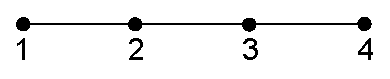
\includegraphics[width=60mm]{Elt1D-ass.eps}
\caption{Discrétisation de la barre en trois éléments}\label{fig-ex2ass}
\end{figure}
\medskipvm
Chaque élément~$e$ (de longueur~$L_e$) possède une matrice de rigidité élémentaire~$\MM{k_e}$ et un vecteur des forces nodales élémentaires~$\VV{f_e}$ définis par:
\begin{equation}
\MM{K_e} = \frac{2EA}{L_e} \MM{\begin{array}{cc} 1 & -1\\ -1& 1 \end{array}}
\qquad \text{ et } \qquad
\VV{f_e} = \rho g A \frac{L_e}4 \VV{\begin{array}{c} 1 \\1 \end{array}}
\end{equation}
\medskipvm
Les variables nodales sont~$\LL{q}=\LL{u_1, u_2, u_3, u_4}$, et, les matrices élémentaires
redonnées ci-dessus s'écrivent, en fonction de ces variables nodales:
\begin{equation*}
\MM{K}_1 = \frac{2EA}{L_1} \MM*{1 & -1 & 0 & 0\\ -1& 1 & 0 & 0\\ 0&0&0&0\\0&0&0&0}
\quad
\MM{K}_2 = \frac{2EA}{L_2} \MM*{0&0&0&0\\ 0& 1 & -1 & 0\\ 0 & -1& 1& 0\\0&0&0&0}
\quad
\MM{K}_3 = \frac{2EA}{L_3} \MM*{0&0&0&0\\0&0&0&0\\0& 0& 1 & -1\\ 0&0 & -1& 1}
\end{equation*}
et les forces nodales:
\begin{equation*}
\VV{f_1} = \rho g A \frac{L_1}4 \VV*{1 \\1\\0\\0}
\quad
\VV{f_2} = \rho g A \frac{L_2}4 \VV*{0\\1 \\1\\0}
\quad
\VV{f_3} = \rho g A \frac{L_3}4 \VV*{0\\0\\1 \\1}
\end{equation*}
\medskipvm
L'\textcolorblue{assemblage} permettant de constituer le système complet est simplement obtenu par:
\begin{equation} \MM{K}=\MM{K}_1+\MM{K}_2+\MM{K}_3 \qquad \text{ et } \qquad \VV{F}=\VV{f_1}+\VV{f_2}+\VV{f_3} \end{equation}
\medskipvm
On résout alors~$\MM{K}\VV{q}=\VV{f}$ avec la condition aux limites~$u_1=0$.

\medskip
\paragraph{Remarque}
La matrice~$\MM{K}$ obtenue sur cet exemple a un \textcolorblue{caractère bande} (la matrice est vide en dehors d'une zone centrée sur la diagonale). Ceci est dû à la numérotation des nœuds. Une autre numérotation pourrait faire perdre ce caractère important (stockage et résolution).

C'est pourquoi, dans les programmes éléments finis, une étape de renumémoration automatique des nœuds est généralement faite.

\medskip
\subsection{Élément de barre unidimensionnel de type Hermite (élément subparamétrique)}\index[aut]{Hermite (Charles), 1822-1901, Français}\index{élément fini!d'Hermite}

En restant encore sur notre élément linéaire unidimensionnel, nous allons voir comment ajouter des contraintes sur les dérivées aux nœuds, comme illustré à la figure~\ref{fig-ex2Her}.
\begin{figure}[ht]\centering
\subfloat[Élément de référence]{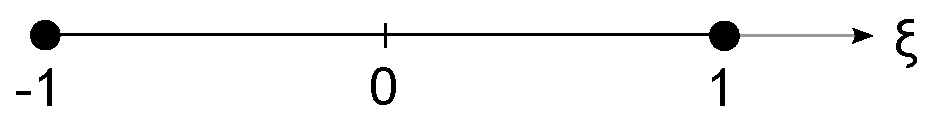
\includegraphics[width=60mm]{Elt1D-ref.eps}} \hspace{5em}
\subfloat[Segment réel (2 nœuds, 4ddl)]{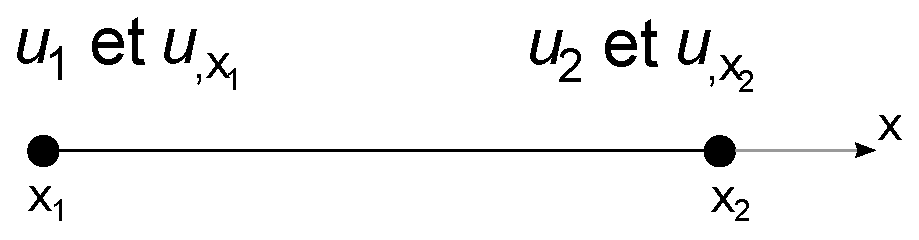
\includegraphics[width=60mm]{Elt1D-hermite.eps}}
\caption{Élément de barre unidimensionnel de type Hermite}\label{fig-ex2Her}
\end{figure}
\medskipvm
La géométrie est encore une fois approximée par:
\begin{equation} x=\frac{1-\xi}2 x_1 + \frac{1+\xi}2 x_2, \quad \xi\in[-1;1] \end{equation}
\medskipvm
Mais cette fois, l'approximation de la fonction solution est voulue sous la forme:
\begin{equation}
u = \LLL{N_1, N_2, N_3, N_4}\VV{u_n} \qquad \text{ avec les ddl } \qquad
\LL{u_n}=\LLL{u_1, u_{,x_1}, u_2, u_{,x_2}} 
\end{equation}
\medskipvm
Les fonctions~$N_i$ choisies sont des fonctions cubiques de type Hermite assurant une continuité de~$u$ et~$u_{,x}$ aux nœuds 1 et 2. On a:
\begin{equation}
N_1=\frac14(1-\xi)^2(2+\xi); \qquad
N_2=\frac{L}8(\xi^2-1)(1-\xi); \qquad
N_3=\frac14(1+\xi)^2(2-\xi); \qquad
N_2=\frac{L}8(\xi^2-1)(1+\xi)
\end{equation}
\medskipvm
Le champ~$u_{,x}$, qui est la déformation~$\varepsilon$ est donné par:~$\varepsilon=\LL{B}\{u_n\}$ avec:
\begin{equation} \LL{B}=\LLL{\frac3{2L}(\xi^2-1), \quad \frac14(3\xi^2-2\xi-1), \quad \frac3{2L}(1-\xi^2), \quad
\frac14(3\xi^2+2\xi-1)}\end{equation}
\medskipvm
La contrainte, dans le cas où le coefficient d'élasticité~$H$ est constant est donnée par:
\begin{equation}\sigma_x=H \LL{B}\VV{u_n}\end{equation}

\medskip
\subsection{Élément mixte unidimensionnel}

Continuons avec notre élément de référence linéaire unidimensionnel. Cette fois-ci nous souhaitons le mettre en relation avec un segment réel dont les inconnues nodales sont les déplacements $u_1$ et~$u_2$, mais qui possède en plus une approximation constante de la contrainte par élément, comme montré sur la figure~\ref{fig-ex2mixte}.
\begin{figure}[ht]\centering
\subfloat[Élément de référence]{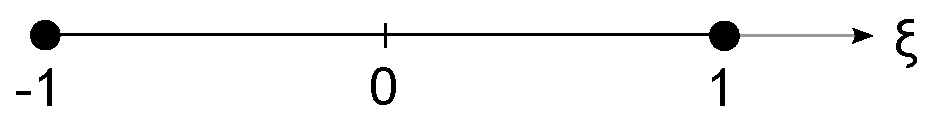
\includegraphics[width=60mm]{Elt1D-ref.eps}} \hspace{5 em}
\subfloat[Élément réel]{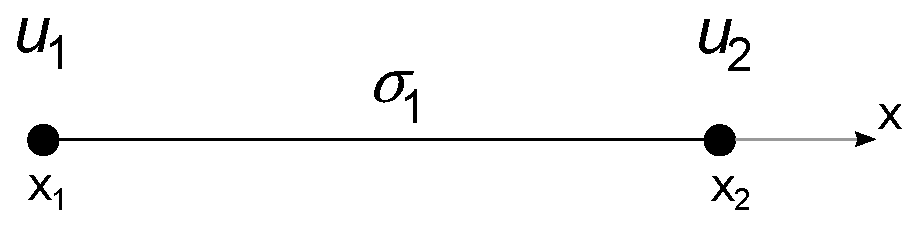
\includegraphics[width=60mm]{Elt1D-mixte.eps}}
\caption{Élément mixte unidimensionnel}\label{fig-ex2mixte}
\end{figure}
\medskipvm
Nous cherchons donc une approximation~$C^0$ du déplacement et~$C^{-1}$ de la
contrainte.
\medskipvm
Pour la géométrie, nous avons une fois encore:
\begin{equation} x=\frac{1-\xi}2 x_1 + \frac{1+\xi}2 x_2, \quad \xi\in[-1;1] \end{equation}
\medskipvm
Pour la contrainte, nous avons:
\begin{equation} \sigma_x(x)=\sigma_1 \text{ (constante)} \end{equation}
\medskipvm
La formulation variationnelle mixte de l'élasticité linéaire unidimensionnel est (voir fonctionnelle
d'Hellinger-Reissner sous sa deuxième forme ou fonctionnelle mixte):\index[aut]{Reissner (Max Erich, dit Eric), 1913-1996, Américain}\index[aut]{Hellinger (Ernst David), 1883-1950, Allemand}\index{fonctionnelle!d'Hellinger-Reissner}\index{fonctionnelle!mixte}
\begin{equation}
W=\dint_0^L A\left(-\sigma_x^*\frac1H\sigma_x+\sigma_x^*u_{,x}+v_{,x}\sigma_x\right) \dd x
-\dint_0^L Avf_x \dd x - (v f_S)_{S_f} = 0\qquad \forall v,\sigma^*
\end{equation}
avec les conditions aux limites~$u=\overline{u}$ et~$u^*=0$ sur~$S_u$.
\medskipvm
De manière discrétisée, il vient:
\begin{equation}
W = \LLL{v_1, v_2, \sigma_1^*}\left(
\MM*{\mO & \VV{b}\\ ~\\ \LL{b} & -a}
\VV*{u_1\\u_2\\ \sigma_1}
- \VV*{\VV{f_n}\\~\\ \sigma_1}
\right)\end{equation}
avec:
\begin{equation}
\VV{b}=\dint_0^L \frac{A}L \VV*{-1\\1}; \qquad
a=\dint_0^L \frac{A}H \dd x; \qquad
\VV{f_n} = \dint_{-1}^{+1} A \VV*{N_1\\N_2} \frac{L}2 f_x \dd\xi =
 A f_x \frac{L}2 \VV*{1\\1}
\end{equation}
\medskipvm
On pourrait s'arrêter là avec le système précédent à résoudre. Toutefois, $\sigma_1$ est une variable locale sans couplage avec les autres éléments. On peut donc l'exprimer en fonction des autres degrés de liberté de l'élément~$u_1$ et~$u_2$. La dernière ligne du système donne:
$\sigma_1^*=\left(\LL{b}\VV{u_n}-a\sigma_1\right)=0$, $\forall \sigma_1^*$,
d'où:
\begin{equation} \sigma_1 = \frac1a \LL{b}\VV{u_n} \end{equation}
\medskipvm
Et le système devient alors:
\begin{equation} W=\LL{v_n}\left( \VV{b}\sigma_1 -\VV{f_n}\right) =
\LL{v_n} \left( \MM{K}\VV{u_n}-\VV{f_n}\right) \end{equation}
avec:
\begin{equation} \MM{K}=\VV{b}\frac1a\LL{b} \end{equation}
Dans le cas où~$H$ est constant, la matrice de rigidité obtenue est identique à celle du modèle en déplacements du paragraphe~\ref{Sec-barre1D}.
